\documentclass[a4paper,11pt]{report}

% General tools
\usepackage{etoolbox}
\usepackage{color}
\usepackage[utf8]{inputenc}
\usepackage{minted}
% Fonts
\usepackage[T1]{fontenc}

% LaTeX modern fonts
\usepackage{lmodern}

% Sans serif
%\usepackage{tgheros}

% Serif
%\usepackage[bitstream-charter]{mathdesign}

% Monospace
%\usepackage{sourcecodepro}

% Language
\usepackage[english]{babel}
\usepackage{blindtext}
\usepackage{url}

% Page style
\usepackage{fullpage} % page margins to 1.5cm
\usepackage{fancyhdr} % headers and footers

% Colors & graphics
\usepackage[table]{xcolor}    % colors
\usepackage[pdftex]{graphicx} % graphics importing

% Misc
\usepackage{titlesec} % section titles formatting
\usepackage{minted}   % code highlighting
\usepackage{lscape}   % landscape
\usepackage{tikz}     % charts in LaTeX
\usepackage{amsmath}  % better math
\usepackage{float}    % floats
\usepackage[small,justification=centering]{caption}
\usepackage{microtype} % typographic improvements

% Paragraphs
\usepackage{parskip}
\usepackage[defaultlines=3,all]{nowidow}

% Chapter titles
% Remove space before title
\titlespacing{\chapter}{0pt}{*-4}{*3}
% Remove "Chapter N" and use a sans-serif font
\titleformat{\chapter}[hang]{\bf\huge}{\thechapter}{1pc}{}
% Change chapter page style
\patchcmd{\chapter}{plain}{fancy}{}{}

% Tables
\usepackage{multirow}

% Cross-references
\usepackage[hidelinks]{hyperref}


% Metadata for this report
% ------------------------
\newcommand{\School}{University of Applied Sciences Western Switzerland}
\newcommand{\Faculty}{MSE - Software Engineering}
\newcommand{\Place}{Lausanne}

% Course

\newcommand{\Title}{<Title>}

% Supervisors (professors)
\newcommand{\Supervisors}{Prof. Carlos Peña}

% Students
\newcommand{\Authors}{Déruaz Vincent}

%TOOLS
\newcommand{\todo}[1]{\textcolor{red}{TODO: #1}\PackageWarning{TODO:}{#1!}}

\newcommand{\Course}{Pa \\ Inphinity}


% Header and footer
% -----------------
\pagestyle{fancy}
\lhead[]{\Course}
\chead[]{}
\rhead[]{\Place, \today}

\setlength{\headheight}{14pt}
\setlength{\headsep}{14pt}

\newcommand{\HRule}{\rule{\linewidth}{0.5mm}}

% Code styles for highlighting
% ----------------------------

% How to use (replace 'java' with language name):
% - code blocks:
%     \begin{javacode}
%     CODE
%     \end{javacode}
% - files:
%     full: \javafile{PATH}
%     extract: \javafile[startline=x, endline=y]{PATH}
% TODO: inline?

% Java
\newminted{java}{frame=single, framesep=6pt, breaklines=true, fontsize=\scriptsize}
\newmintedfile{java}{frame=single, framesep=6pt, breaklines=true, fontsize=\scriptsize}

% Scala
\newminted{scala}{frame=single, framesep=6pt, breaklines=true, fontsize=\scriptsize}
\newmintedfile{scala}{frame=single, framesep=6pt, breaklines=true, fontsize=\scriptsize}

% Python
\newminted{python}{frame=single, framesep=6pt, breaklines=true, fontsize=\scriptsize}
\newmintedfile{python}{frame=single, framesep=6pt, breaklines=true, fontsize=\scriptsize}

% Plain text
\newminted{text}{frame=single, framesep=6pt, breaklines=true, breakanywhere, fontsize=\scriptsize}
\newmintedfile{text}{frame=single, framesep=6pt, breaklines=true, breakanywhere, fontsize=\scriptsize}

% Document
% --------
\begin{document}

\begin{titlepage}
\begin{flushright}
\begin{minipage}{0.5\textwidth}
\begin{flushleft}

\includegraphics[width=0.9\textwidth]{./img/mse_logo}
\end{flushleft}
\end{minipage}%
\begin{minipage}{0.5\textwidth}
\begin{flushright}

\includegraphics[width=0.6\textwidth]{./img/logo_hes-so}
\end{flushright}
\end{minipage}
\begin{flushleft}
\footnotesize
Master of Science HES-SO in Engineering \\
Av. de Provence 6 \\
CH-1007 Lausanne
\end{flushleft}
~\\[0.5cm]

\huge Master of Science HES-SO in Engineering\\[0.5cm]

\large Orientation : Technologies de l’information et de la communication(TIC)\\[0.5cm]
~\\[1cm]
% Title
{
\Huge PA - Inphinity \\[1.5cm]
}
{
Done by:\\
\huge Déruaz Vincent\\[0.5cm]
}
{
Under the supervision of: \\
Prof. Carlos Peña \\
of HEIG-VD
}
\vfill

% Bottom of the page
{Lausanne, HES-SO//Master, \today}

\end{flushright}
\end{titlepage}

\newpage
\mbox{}

\vspace{0.5cm}
{
\huge Accepted by HES SO//Master (Suisse, Lausanne) \\
\huge On a proposal from\\
\huge Prof. Carlos Peña, Pa advisor
}

\vspace{8cm}
\textbf{Advisor} \\
Prof. Carlos Peña \\
of HEIG-VD

\vspace{3cm}
\textbf{MRU responsable} \\
Prof. Eduardo Sanchez \\
of HEIG-VD
\newpage

\tableofcontents


\chapter{Introduction}
\section{foreword}
This project falls within the context of a thesis proposed by Prof. Carlos Peña, YokAi
Que, MDPhD and Grégory Resch, PhD entitled \textit{In silico prediction of phagebacteria
infection networks as a tool to implement personalized phage therapy} \cite{ref1}.

The official statment of the project is:\\
By using automated learning methods, explore alternative methodologies for bacteria and phages interaction modelisation on genomic information or proteins.


\section{phages Vs bacteria}
In our modern world a challenging issue has appeared concerning conventional antibiotics. In deed, some bacteria have developp resistance to antibiotics. To overcome this, people are looking at phage therapy. 

Phage therapy is the utilisation of phages, bacteriophage virus, to treat infectious diseases of bacterial origin. Phage, also called bacteriophage, are a specific type of virus infecting only bacteria. This therapy is known to have only very few and only benign side effects. This last point make phagotherapy, not only useful to avoid antibiotic in case of resistance, but also to avoid their "toxicity".

Briefly, phage therapy was the only treatment solution before the 1930's. The appearence of the penicillin in the early 1940's and other modern drugs, relegate phage therapy to the past. But, in the slavic countries, phage therapy continued to be used as a current treatment.

Luckily for us, we don't have to start from nothing in phage therapy. However, we have the necessity to find a way, a methode to validate the phage selection. \cite{ref2}


\chapter{Theories}
This chapter is made to ensure that every reader understands basics needed. It contains some simplifications and it's not, in any case, a biology guide.
\vspace{-0.6cm}
\section{Biology}
Before entering in the project content, let's say some words about genomic. Almost all living organisms use \textbf{Deoxyribonucleic acid, DNA,} \cite{ref9}. DNA contains the necessary information for the developpment and activities of living creatures.

\begin{figure}[H]
\centering
\begin{minipage}{.5\textwidth}
  \centering
  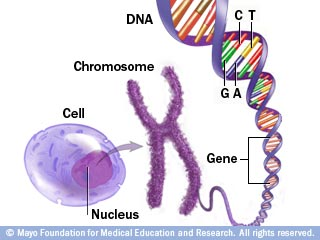
\includegraphics[width=.8\linewidth]{img/chromosome}
  \captionof{figure}{DNA visualisation}
  \label{fig:test1}
\end{minipage}%
\begin{minipage}{.5\textwidth}
  \centering
  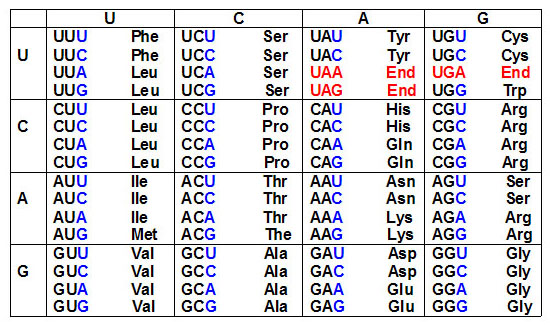
\includegraphics[width=.7\linewidth]{img/geneticcode}
  \captionof{figure}{Codons to proteins}
  \label{fig:test2}
\end{minipage}
\end{figure}

DNA is composed of 4 units, called nucleotide bases, adenine (A), thymine (T), guanine (G), and cytosine (C). Those bases are stored in chromosomes, in human cells (Fig 2.1). They are responsible for coding information used to create proteins (Fig. 2.2). Organisms structural organisation and every biological activity are made up from proteins.
\vspace{-0.6cm}
\section{Bio-informatic}
\vspace{-0.6cm}
\subsection{DNA sequencing}
\vspace{-0.2cm}
Today we are capable of sequencing genetical code of any organism. When DNA is sequenced, only one half is recorded, because every base work in pairs (C-G | T-A). With all available phages and bacteria sequenced, we have enormous data at our disposal.

\textbf{Note:} For more information about sequencing see article in reference \cite{ref9}.

\subsection{Phamily}
\vspace{-0.2cm}
A pham is a collection of protein-coding genes whose related sequence, determined by pairwise analysis, are used for comparison. Sequence alignment is used to determin conserved domain in DNA of phage. A phamily contains all related genes.

\subsection{Genbank}
\vspace{-0.2cm}
Most of the genetic information used in this project can be found on GenBank \cite{ref10}. GenBank is a public database regrouping avalaible DNA sequences and information.


\chapter{Methods}
In this section we will discuss about what we've used during this project. The Docker technology is used to build the different work environment. Phamerator and PhamDB are used to compute genomes into phamily. Everything is stored into some Sql databases.

\section{Docker}
Docker allows to package applications with a functional system and every dependency needed to run it, into a standardized container. \cite{ref3} You run those containers host machine using a docker-machine (docker engine). 

\subsection{Functionment}
In a specific file called 'Dockerfile' you describe a system. You can build and run this system everywhere docker engine is installed. It will create a container, containing your application.

Containers are an isolated system from host or other containers. You can use every Linux distribution to run your container.

Docker build images using layers, it allows docker to share those layers between containers, reducing disk use at best.

\begin{figure}[H]
	\begin{center}
		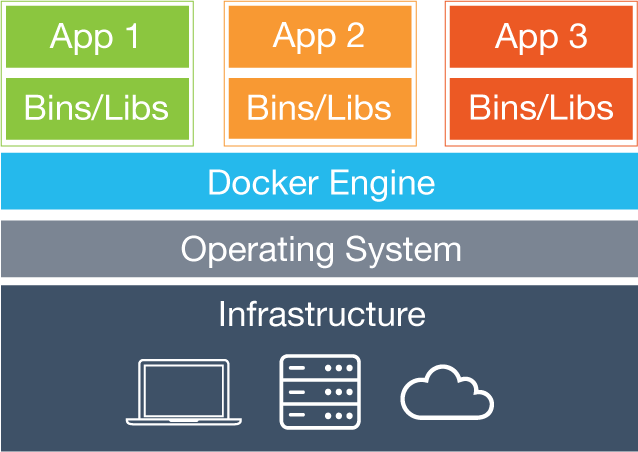
\includegraphics[scale=0.35]{img/what-is-vm-diagram}
		\caption{Docker harchitecture}
	\end{center}
\end{figure}
\newpage
\subsection{Docker-machine installation}
you have to install docker on your system, it can be used on Linux, Windows or MacOs. \url{https://docs.docker.com/linux/}

\subsubsection{Windows}
If you want to use docker on Windows you need to do as following to ensure to have a docker-machine with more than 20Go.

\begin{javacode}
$ docker-machine rm default
$ docker-machine create -d virtualbox --virtualbox-memory=4096 --virtualbox-cpu-count=2 --virtualbox-disk-size=50000 default
\end{javacode}

It will create a docker-machine with 50Go of disk space.

\subsection{Docker commands}
Here are the basic commands you will need to manage docker. Be careful, you will need to be in the same directory as the Dockerfile.

This command allow to build an image described in the Dockerfile.
\begin{javacode}
$ docker build -t "<image Name>" .
\end{javacode}

This command is used to run a container using a pre-build image, with a binding port.
\begin{javacode}
$ docker run -it -d -p <host port>:<container port> <image name>
\end{javacode}

If you need to access the container bash console, just use this command
\begin{javacode}
$ docker exec -i -t <container ID> /bin/bash
\end{javacode}

You can list all the running containers and use a <container id> to stop it.
\begin{javacode}
$ docker ps
$ docker stop <container ID>
\end{javacode}

This last command give you the ip of your docker-machine.
\begin{javacode}
$ docker-machine ip
\end{javacode}
\newpage
\subsection{Inphinity, build \& run}
For the main code of this project we use python through Jupyter. To do so you can find a docker image that run Jupyter, python3 and some machin learning libraries. go to "dockers/jupyter\_align\_mysql" directory.

To build and run the environment, type the following commands:
\begin{javacode}
$ docker build -t "pa/inphinity" .
$ docker run -v <path to project dir>/jupyter_align_mysql/src:/home/pa/work/ -i -t -d -p 8888:8888 pa/inphinity
\end{javacode}

Replace <path to project dir> by the entire path to the directory. If you want to, you can change the host port. Just change "\textit{-p 8888:8888}" to "\textit{-p <any port>:8888}".

You can now access the jupyter interface and the project files using any browser you want using \url{http://<docker-machine ip>:8888}

At this point you should see the interface figure 3.2

\begin{figure}[H] 
	\begin{center}
		
\includegraphics[scale=0.45]{img/login_jupyter}
		\caption{Jupyter login page}
	\end{center}
\end{figure}

\textbf{Rq:} The password is "Inphinity-more"

When you're logged in you can access the "inphinity" directory. It contains most of this project results. We will discuss them later in this document.

\begin{figure}[H] 
	\begin{center}
		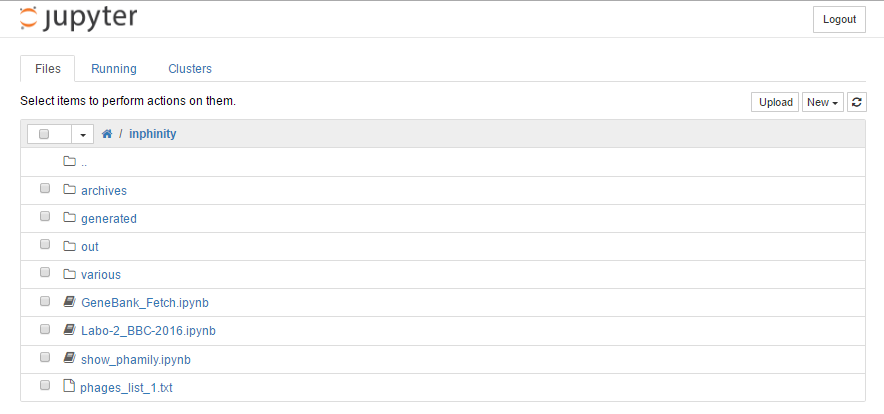
\includegraphics[scale=0.45]{img/inphinity_jupyter}
		\caption{Inphinity jupyter directory}
	\end{center}
\end{figure}
\newpage
\section{Phamerator}
Phameraotr is \textit{a bioinformatic tool for comparative bacteriophage genomics} \cite{ref4}. Phamerator will allow us to compute and store phamily, in a database. 

\subsection{Installation}
To use phamerator you have to install a linux environment. Thus copy the file "phamerator.sh" from the directory and execute it in order to install and run Phamerator.

Normally your Phamerator should start at the end (Fig 3.4).

\begin{figure}[H] 
	\begin{center}
		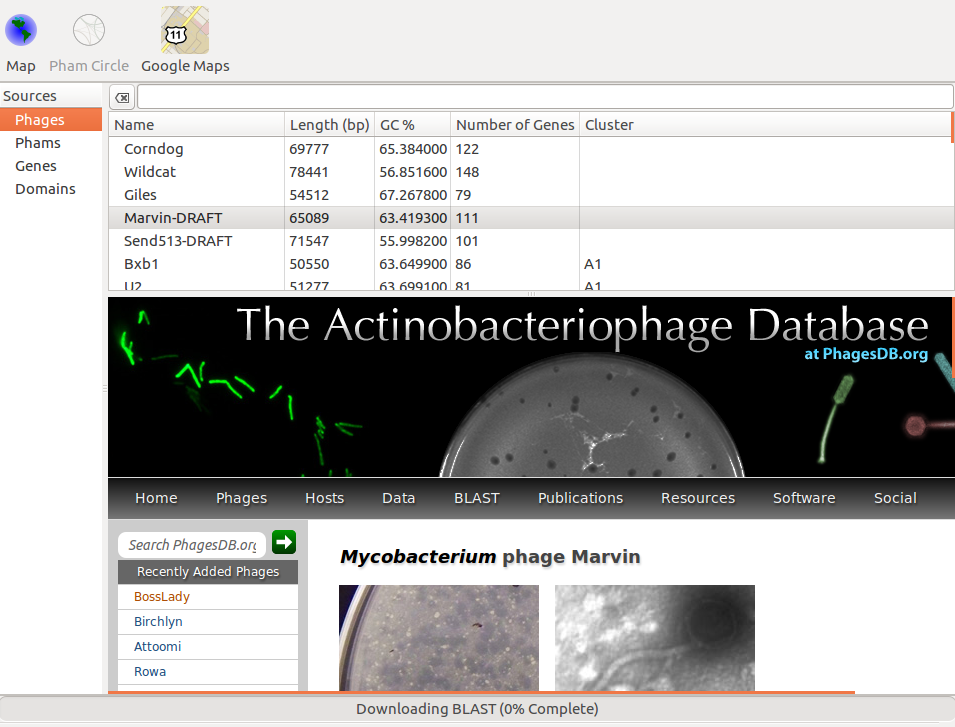
\includegraphics[scale=0.3]{img/phamerator_1}
		\caption{phamerator interface 1}
	\end{center}
\end{figure}

\subsection{How it's works}

Phamerator starts with a default database, \textit{SEA - phamerator.csm.jmu.edu}. Wich we will use in this project and modify. You can change the database source from menu \textit{Edit --> Preferences --> Network --> Server/Database}.

\begin{figure}[H] 
	\begin{center}
		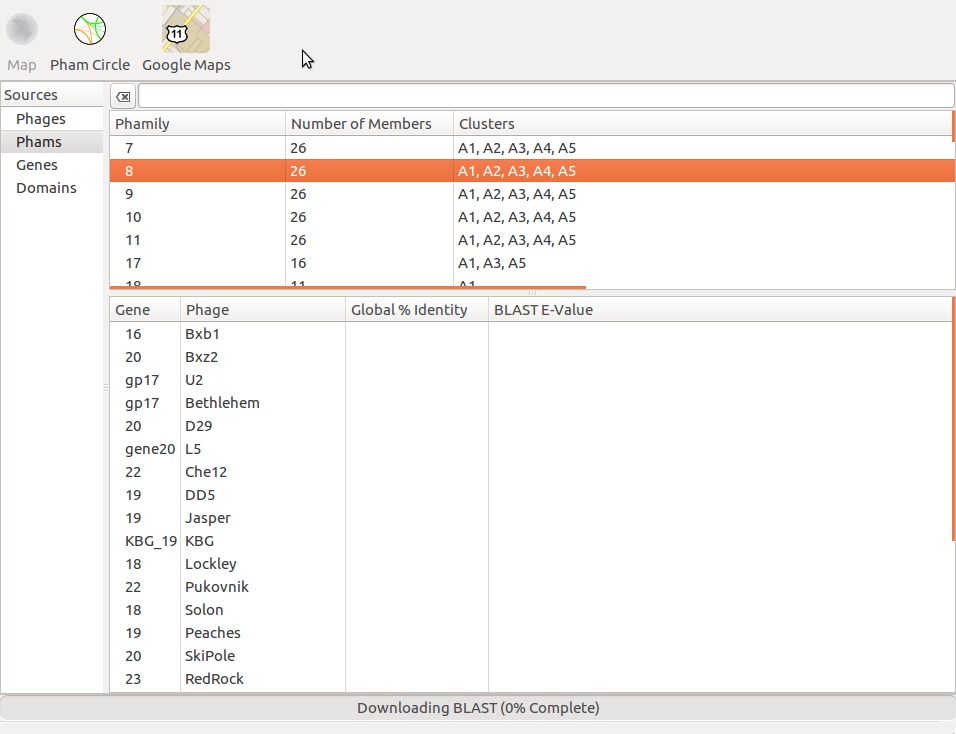
\includegraphics[scale=0.3]{img/phamerator_2}
		\caption{phamerator interface 2}
	\end{center}
\end{figure}

As you can see on figure 3.5, you can choose to display information about phages, phams, genes or domains. In our case we are more interested by phams. We can see every pham on the database and order them by name, number of members or clusters. Keep in mind that you can consult them ordered by number of members from Phamerator when reading section 3.5.2.

\begin{figure}[H] 
	\begin{center}
		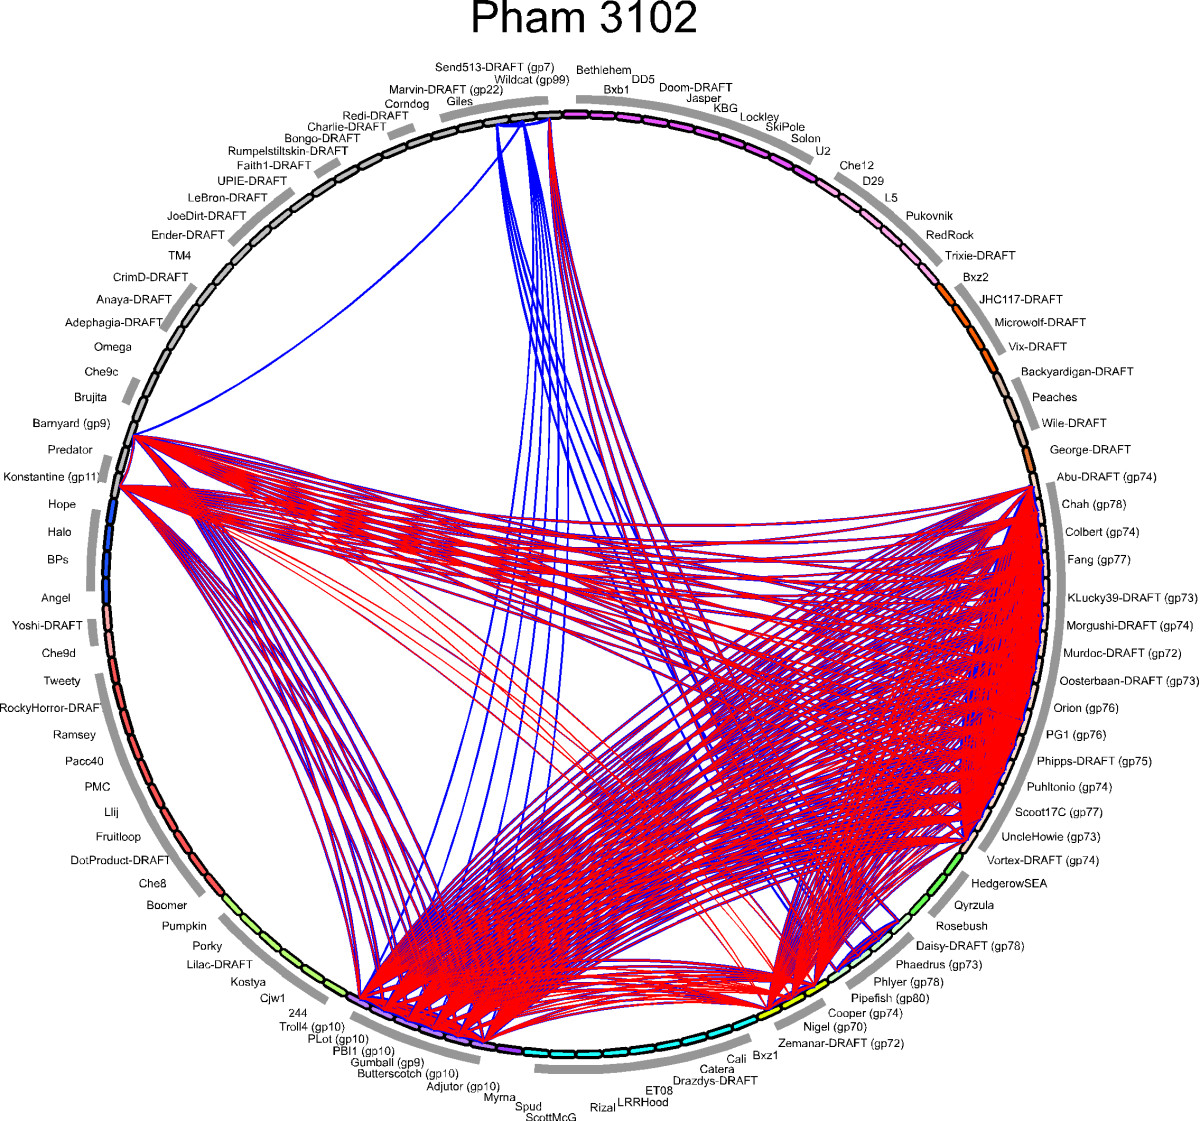
\includegraphics[scale=0.45]{img/12859_2011_Article_4954_Fig8_HTML}
		\caption{phamerator interface 3}
	\end{center}
\end{figure}

Pham Circle give you a graphical overview of the selected pham. It give you a view of horizontal genetic exchange between phage in evolution.

\section{PhamDB}
To facilitate the construction of databases containing our phamily we will use PhamDb. In deed, with phamDb we can populate a database with new phage. At every addition of phage, it will recompute phamily accordingly to the new phage added. 

We no longer need to access to Phamerator by GUI. In the future it will let us build a fully automated pipline of actions.

\subsection{Installation \& Run}
To build and run the environment type the following commands:
\begin{javacode}
$ docker build -t "pa/phamdb" .
$ docker run -v <path to project dir>/jupyter_align_mysql/src:/home/pa/work/ -i -t -d -p 81:80 pa/phamdb
\end{javacode}

Replace <path to project dir> by the entire path to the directory. If you want to, you can change the host port. Just change "\textit{-p 81:80}" to "\textit{-p <any port>:80}".

You can now access the jupyter interface and the project files using any browser you want using \url{http://<docker-machine ip>:80}
\newpage
At this point you should see the interface figure 3.7, but with no database for the moment.

\begin{figure}[H] 
	\begin{center}
		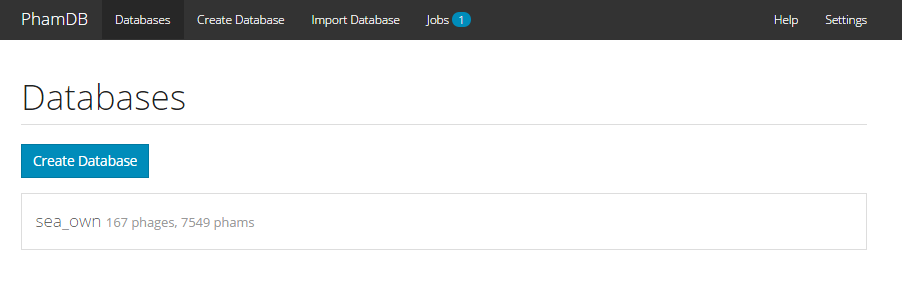
\includegraphics[scale=0.45]{img/phamdb}
		\caption{Phamdb interface}
	\end{center}
\end{figure}

\subsection{Utilisation}
As you see from figure 3.8 you can access the list of all existing databases and consult them.

\begin{figure}[H] 
	\begin{center}
		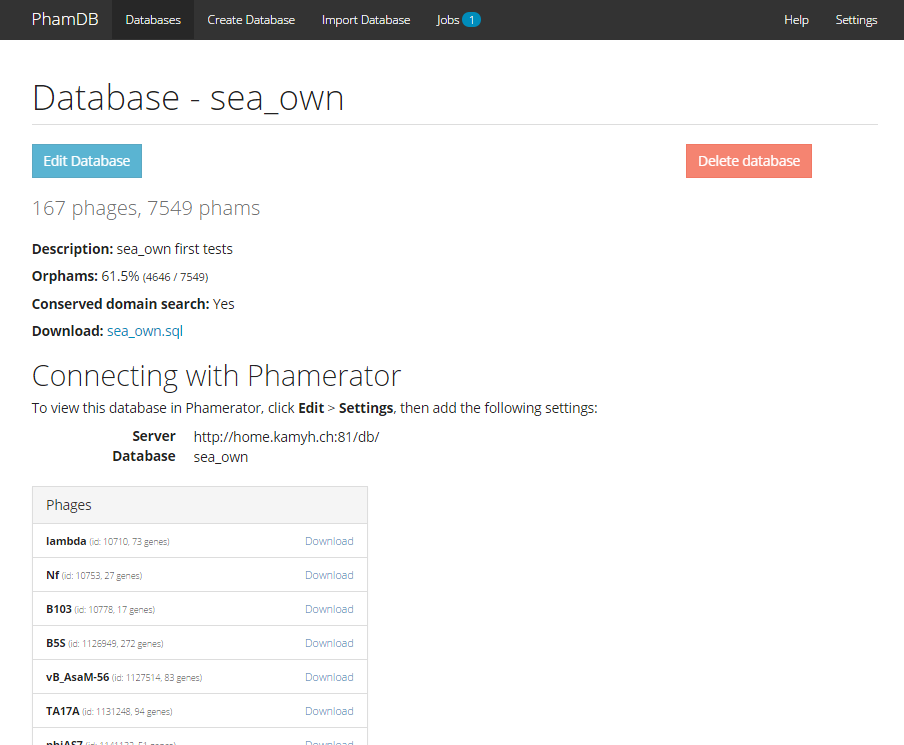
\includegraphics[scale=0.45]{img/phamdb_see_db}
		\caption{PhamDb database visualisation}
	\end{center}
\end{figure}

You can create a new database from three different ways:
\begin{enumerate}
	\item By importing phages from existing database on phamdb.
	\item By uploding Genbank files.
	\item By importing as an Sql file.
\end{enumerate}

\begin{figure}[H] 
	\begin{center}
		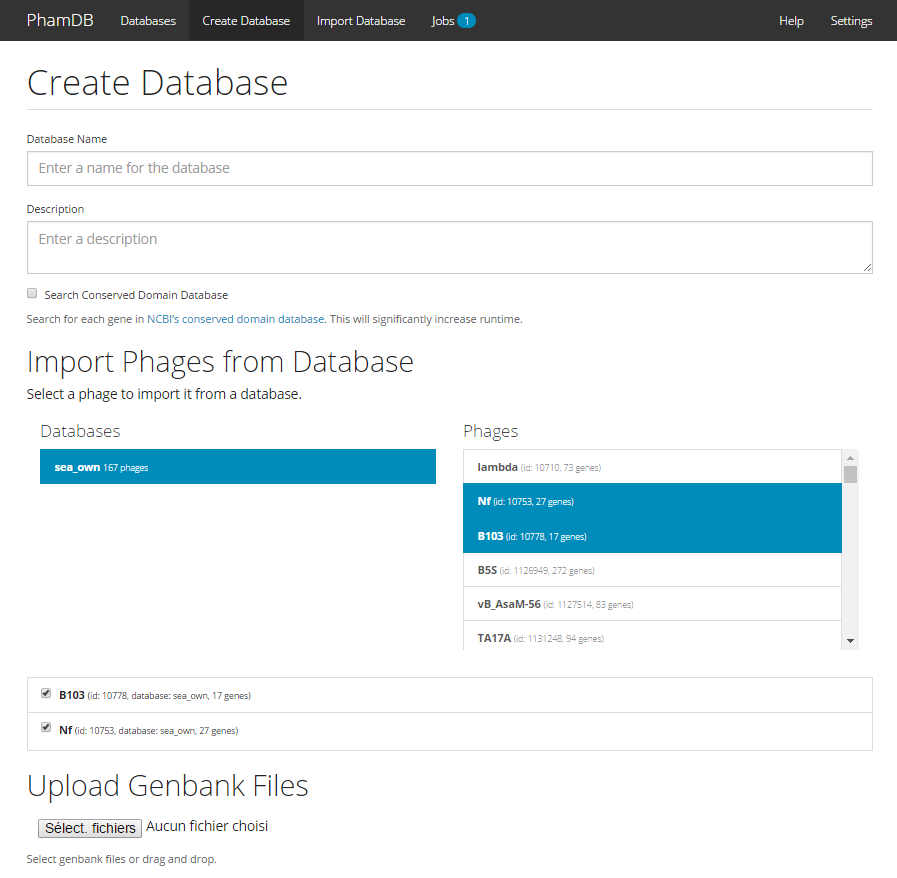
\includegraphics[scale=0.45]{img/phamdb_create_db}
		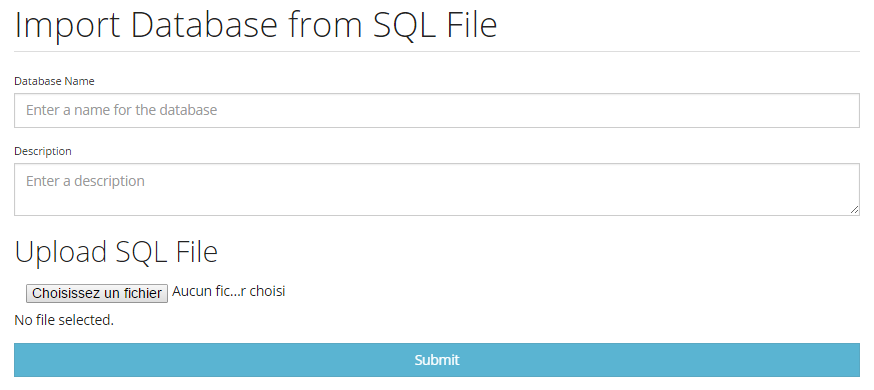
\includegraphics[scale=0.45]{img/phamdb_create_db_2}
		\caption{PhamDb database creation}
	\end{center}
\end{figure}
\newpage
\section{Database \& Dataset}
We use the default database from phamerator for this phase of the project in order to gain some time. You can see the database structure on the figure 3.10 .

\begin{figure}[H] 
	\begin{center}
		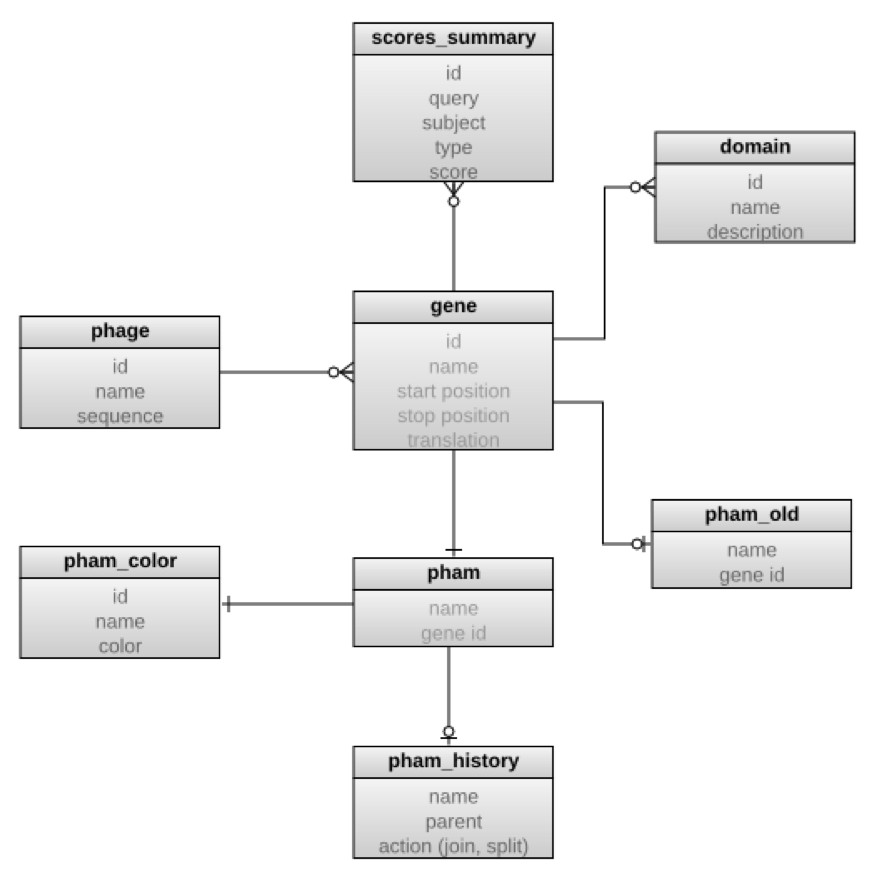
\includegraphics[scale=0.52]{img/12859_2011_Article_4954_Fig1_HTML}
		\caption{Phamerator database architecturea}
	\end{center}
\end{figure}

From the dataset at our disposal, we've used the list of phage "phages\_list\_1.txt". You can find it in annexe of this document.


\section{Phamily}
Now we will discuss about phamily and the main script realised during this phase of the project. You can see and run the following code from the jupyter interface, Cf. chapter 3.1.4.

\subsection{Introduction}

\textbf{Have to:} You are now in your browser and have opened the source file \textit{inphinity/show\_phamily.ipynb}. The class \textit{sea\_inphinity()} has every method that we use in this part. cf. file if you want to see it all.

First we have to create an Inphinity() object capable of access our data. We will use a modified database 'sea\_own', we will discuss his creation later in the document (cf section 4.2.1).

\begin{figure}[H] 
\begin{minted}
[
frame=lines,
framesep=2mm,
baselinestretch=1.2,
bgcolor=lightgray,
fontsize=\footnotesize,
linenos
]
{python}

inphinity = Inphinity('sea_own')
#Result: Number of phages loaded: 167

\end{minted}
\caption{Inphinity object}
\end{figure}

You can display the list of every existing phamily in the database currently selected.

\begin{figure}[H] 
\begin{minted}
[
frame=lines,
framesep=2mm,
baselinestretch=1.2,
bgcolor=lightgray,
fontsize=\footnotesize,
linenos
]
{python}

list_name = inphinity.get_list_name_pham(-1)
print(list_name)
#Result: [... ,2798,2799,2800,2801, ...]

\end{minted}
\caption{Phame names listing}
\end{figure}

\textbf{Note:} A verbosity parameter allows to turn off console message from python execution work flow.

\begin{figure}[H] 
\begin{minted}
[
frame=lines,
framesep=2mm,
baselinestretch=1.2,
bgcolor=lightgray,
fontsize=\footnotesize,
linenos
]
{python}

inphinity.verbose = False

\end{minted}
\caption{Verbosity attribut}
\end{figure}

\subsection{Phages selection}
Now we want to be able to get a philogenetic tree for a phage. To do so we choose a pham, here pham '2799' and we call our method \textit{inphinity.build\_tree('2799')}.

\begin{figure}[H] 
\begin{minted}
[
frame=lines,
framesep=2mm,
baselinestretch=1.2,
bgcolor=lightgray,
fontsize=\footnotesize,
linenos
]
{python}

def build_tree(self,pham):
    genes = self.get_genes_from_a_pham(pham)
    self.create_fasta(genes)
    self.align_muscle()
    self.compute_tree()
    self.prepare_tree_fig()

\end{minted}
\caption{Creation of philogenetic tree}
\end{figure}

As you can see, this methods does a couple of different things. First we're retrieving all the genes composing our pham.
\newpage
Now that we have selected only a few genes, we have to store them into a FASTA file to be used with MUSCLE to align them.

\begin{figure}[H] 
\begin{minted}
[
frame=lines,
framesep=2mm,
baselinestretch=1.2,
bgcolor=lightgray,
fontsize=\footnotesize,
linenos
]
{python}

def create_fasta(self, genes):
    print('Creation of the FASTA file')
    fasta = open("%sfasta.fa" % (self.out_dir), "w")
    self.print_("Number of Genes: %d" % (len(genes)))
    for gene in genes:
        GeneID = gene['GeneID']
        name = gene['Name']
        description = ">%s - %s" % (GeneID, name)

        translation = gene['translation']

        self.print_(description)
        self.print_(translation)

        fasta.write(description)
        fasta.write('\n')
        fasta.write(translation)
        fasta.write('\n')

    fasta.close()

\end{minted}
\caption{FASTA creation function}
\end{figure}

The FASTA file should look like figure 3.16. A gene takes two lines. First the gene identification number and its name. Then, the second line, the gene translation. You can find it in annexe ()

\begin{figure}[H] 
	\begin{center}
		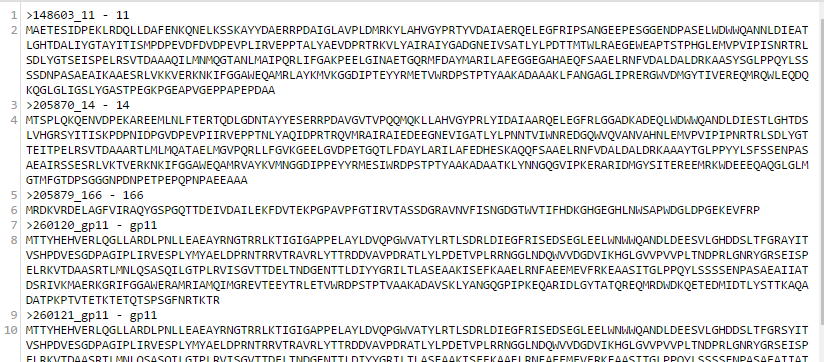
\includegraphics[scale=0.6]{img/fasta}
		\caption{FASTA file}
	\end{center}
\end{figure}

Now we are ready to use MUSCLE to aline genes together. In the future it will be interesting to take some time to customize, with options, our call to MUSCLE \cite{ref5}



\begin{figure}[H] 
\begin{minted}
[
frame=lines,
framesep=2mm,
baselinestretch=1.2,
bgcolor=lightgray,
fontsize=\footnotesize,
linenos
]
{python}

def align_muscle(self):
        print('Alignment with MUSCLE')
        muscle_loc = r'/home/pa/work/muscle3.8.31_i86linux64' # modifier si nécessaire

        muscle_cline = MuscleCommandline(cmd=muscle_loc,input='%sfasta.fa' % 
        	(self.out_dir),out='%sout.aln' % (self.out_dir),clwstrict=True)
        stdout, stderr = muscle_cline()

        muscle_align = AlignIO.read('%sout.aln' % (self.out_dir),'clustal')
        self.print_(muscle_align)

\end{minted}
\caption{Muscle alignment}
\end{figure}

MUSCLE takes our generated FASTA file to produce a .aln file who will contain the alignments.

Now we have our alignments ready to compute a phylogenetic tree. To realise the tree we use \textit{FastTree} software. It will produce "approximately-maximum-likelihood phylogenetic trees" using our .aln file previously generated. 

\begin{figure}[H] 
\begin{minted}
[
frame=lines,
framesep=2mm,
baselinestretch=1.2,
bgcolor=lightgray,
fontsize=\footnotesize,
linenos
]
{python}

def compute_tree(self):
    print('Compute tree')
    AlignIO.convert('%sout.aln' % (self.out_dir),'clustal','%sintermediate.phy' \
    	% (self.out_dir), 'phylip-relaxed')

    cmd_fasttree = r'fasttree'
    fasttree_cmdline = FastTreeCommandline(cmd=cmd_fasttree,fastest=True, \
    	input='%sintermediate.phy' % (self.out_dir),out='%stree.tre' % (self.out_dir))
    out_log, err_log = fasttree_cmdline()

    self.print_('Out Log:')
    self.print_(out_log)

    self.print_('Error Log')
    self.print_(err_log)

    self.tree = Phylo.read('%stree.tre' % (self.out_dir), 'newick')

\end{minted}
\caption{Tree creation}
\end{figure}

\textbf{Note:} As for MUSCLE utilisation, maybe some modification to the call of FastTree can be used to improve the solution.
\newpage
The following figure (3.19) show that we now have a file with our tree. Every genes has a score that will decide for its place in the tree.

\begin{figure}[H] 
	\begin{center}
		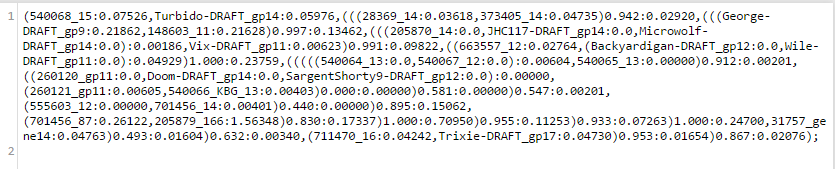
\includegraphics[scale=0.6]{img/tree}
		\caption{Tree score}
	\end{center}
\end{figure}

Now we can compute the visualization of the tree using two functions, \textit{prepare\_tree\_fig()} and \textit{draw\_tree()}.

The function \textit{compute\_tree()} set an attribut, \textit{self.tree}, to \textit{Inphinity()} class. This is our tree, so we can use it after computation. For the selected pham we have the tree from figure 3.20. We will discuss the result in the chapter 4.

\begin{figure}[H] 
	\begin{center}
		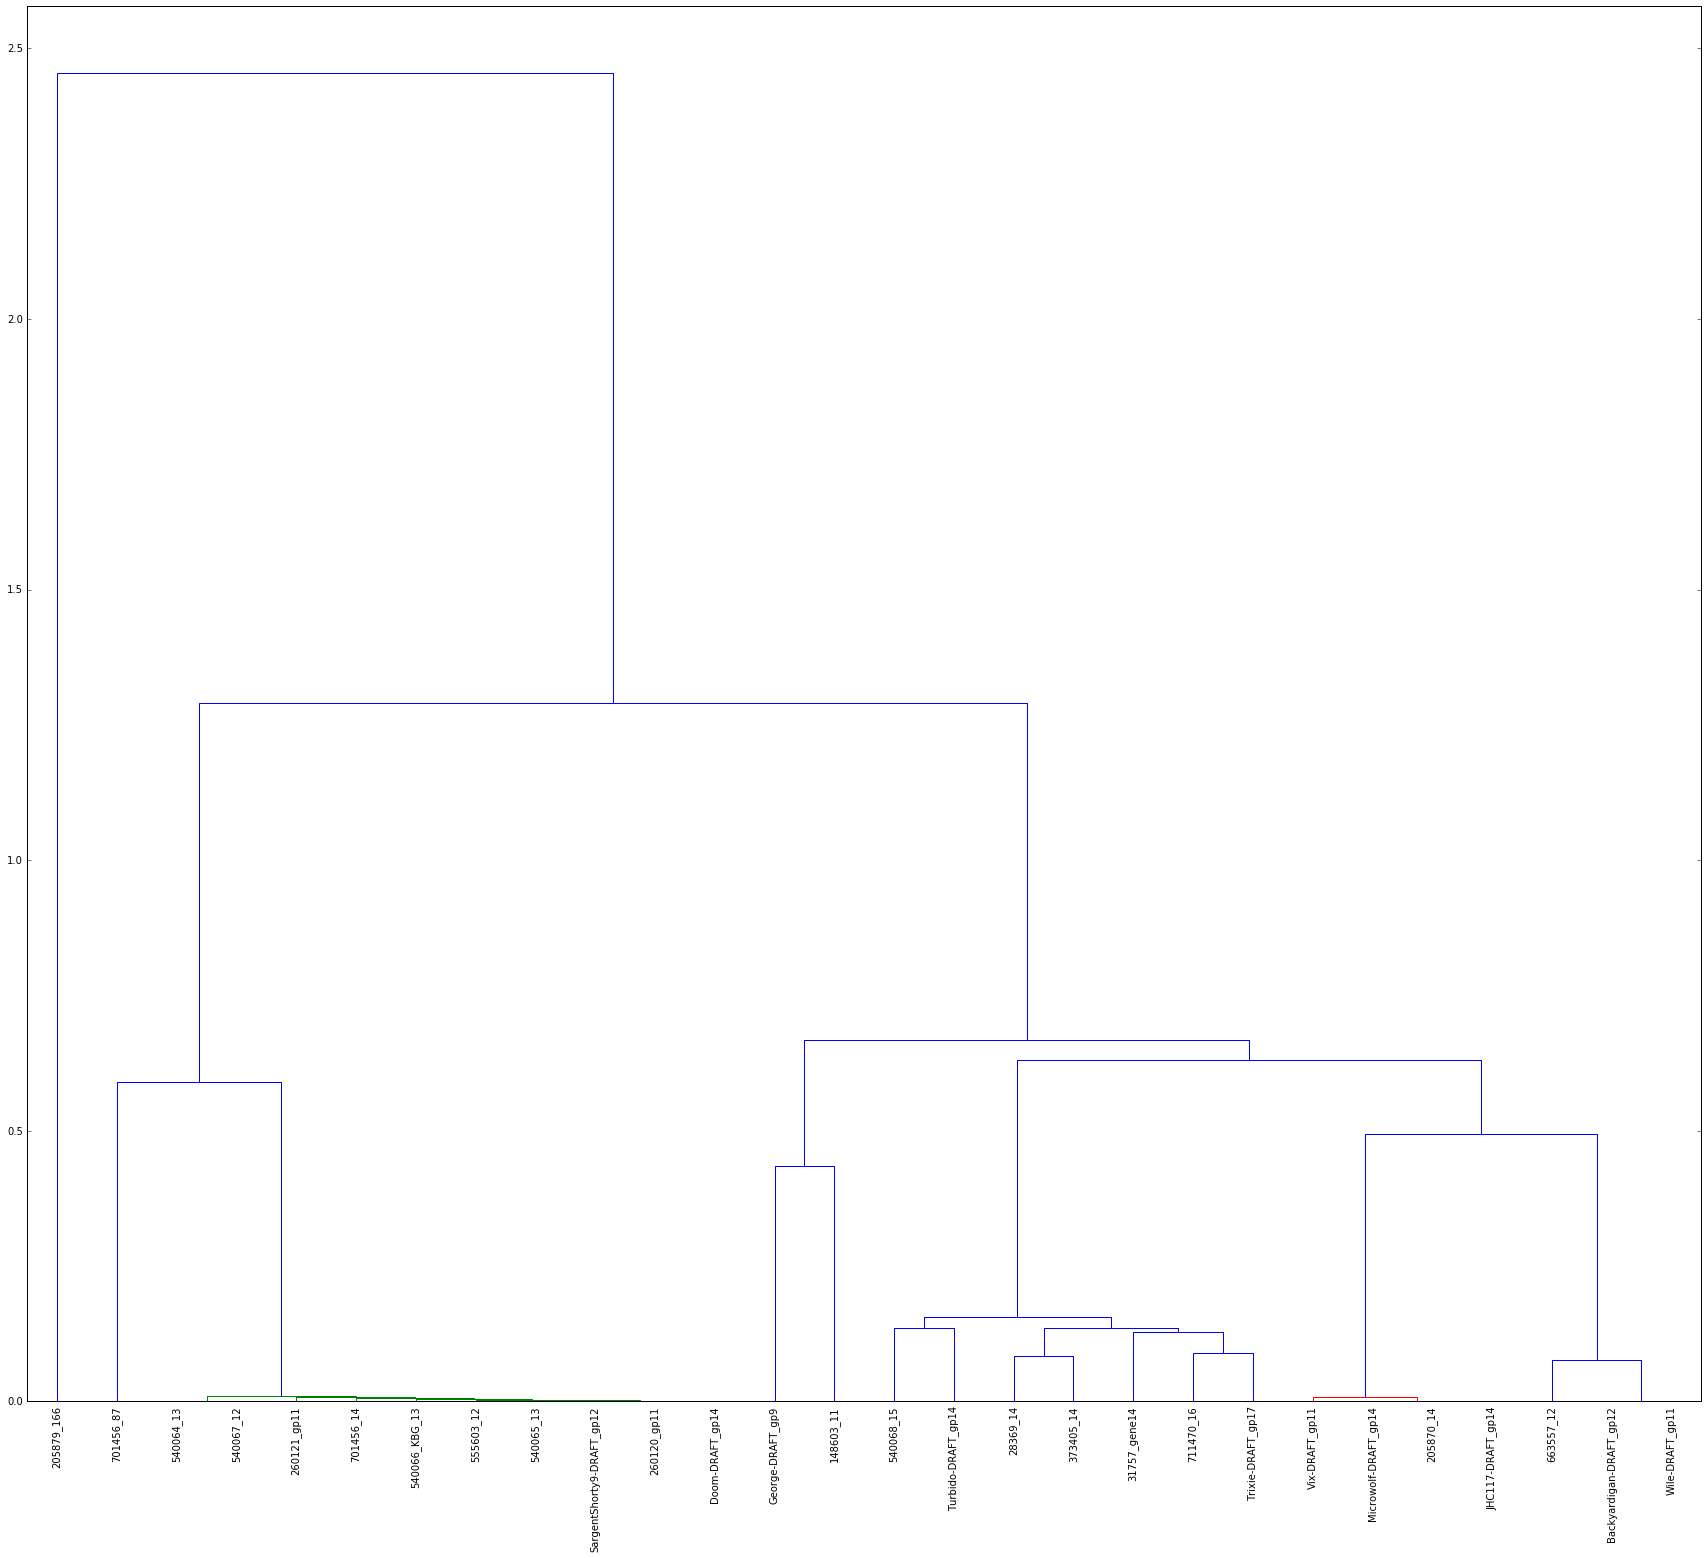
\includegraphics[scale=0.28]{img/tree_fig}
		\caption{Phylogenetic tree}
	\end{center}
\end{figure}
\newpage
\subsection{Displaying results}
you can display information concerning all pages of the selected pham in text format.

\begin{figure}[H] 
\begin{minted}
[
frame=lines,
framesep=2mm,
baselinestretch=1.2,
bgcolor=lightgray,
fontsize=\footnotesize,
linenos
]
{python}

inphinity = Inphinity('sea')
inphinity.verbose = False
inphinity.build_tree('2799')
inphinity.print_informations_on_phages(inphinity.leaves)

\end{minted}
\caption{Information display function}
\end{figure}

We will discuss the content of those information in section 4.1. The avalaible information is the phage gene id who's been used to build the tree, the phage identification number, the phage name, the phage access identifier on Genbank and the phage host strain.

The host strain is labeled in three colors. Blue means that the host strain is known from the loaded database. Red means that host strain information comes from GenBank access. Finally, information is retrieved using webscraping on Phagedb.org.

\subsection{Data completion}
As said in previous section, 3.5.3, the original database was not fully populate. Information about host strain was sometimes missing. In the future we will complete this database but for now, the software retrieve them every time it's needed.

\begin{figure}[H] 
\begin{minted}
[
frame=lines,
framesep=2mm,
baselinestretch=1.2,
bgcolor=lightgray,
fontsize=\footnotesize,
linenos
]
{python}

def get_host_from_genbank(self, genome_id):
    try:
        record = Entrez.efetch(db="nuccore", id=genome_id, rettype="gb", retmode="text")

        filename = 'out/genBankRecord.gb'
        with open(filename, 'w') as f:
            f.write(record.read())
        parsed_gb_file = next(SeqIO.parse(filename, "genbank"))
        return parsed_gb_file.annotations["source"]
    except:
        return 'Not Found'

def get_informations_from_phage_db(self, phage_name):
    page = requests.get('http://phagesdb.org/phages/%s' % (phage_name))
    tree = html.fromstring(page.content)

    host = tree.xpath('//*[@id="phageDetails"]/tbody/tr[2]/td[2]/a/em/text()')[0]

    return host

\end{minted}
\caption{Data completion functions}
\end{figure}

\chapter{Results \& Analyse}

In this chapter we'll talk about the results produced during this project.

\section{First result}
We've not had lots of time to produce and analyze many results and the missing host strain in the data has slowed the work.

We can produce phylogenetic tree for any calculated Pham in database.  For the moment we treat all genes from a tree the same way. See in section 5.2.3 for future developpment.

For better lisibility, scores used in the tree building phase are not directly drawn on it. To display scores, in order to analyze results, use the method from figure 4.1. It give pairwise distances between two leaves.

\begin{figure}[H] 
\begin{minted}
[
frame=lines,
framesep=2mm,
baselinestretch=1.2,
bgcolor=lightgray,
fontsize=\footnotesize,
linenos
]
{python}

def display_scores(self):
    print('Display Scores')

    self.leaves = [str(cladit) for k,cladit in enumerate(self.tree.get_terminals())]
    for l1,leave1 in enumerate(self.leaves):
        for l2,leave2 in enumerate(self.leaves):
            distance = self.tree.distance(leave1,leave2)
            if distance > 0:
                print('-----------------------------')
                print('%s - %s' % (leave1,leave2))
                print(distance)

\end{minted}
\caption{Score display function}
\end{figure}

For pham \textit{2799} we can split the pham into parts using those distances. On figure 3.20 those parts are colored differently depending on their belonging.

Using a figure tree is not really practical to make things automatic. So function \textit{prepare\_tree\_fig} set the attribute \textit{self.leaves}. This attribute stores all genes composing a pham. Using the code from figure 3.21 it shows for all genes, the phage and its host strain.

As you can see in annexe \textit{res\_pham\_2799\_host\_strain.pdf}, every host strain for this pham is \textbf{Mycobacterium smegmatis}.

\textbf{Note:} See issue at section 5.1.2 about phage host strain in the current database.


\section{Database}
\subsection{SEA}
For this phase of the project we've used the \textit{SEA} database \cite{ref7}. This db is populated with 113 phages and 2771 phams.

\textbf{Note:} See in annexes, file \textit{SEA.sql} for the db sql dump.

We've used PhamDb to add some more phages to the database. For now the new database, \textit{SEA\_own}, contains 167 phages and 7549 phams. An issue with PhamDb, cf. section 5.1.3, is responsible for the fact that we've only added 84 new phages.

We've generated a list of phages from \textit{Ebi} \cite{ref8}. A file containing this list has been generated, cf annexes \textit{phages\_list\_1.txt}. Using the code from \textit{inphinity/GeneBank\_Fetch.ipynb} we can store in GenBank files information and sequences about our new phages. 

\section{Linking all together}
We have tree principal parts in thie project. First we have phamerator from where we've taken the original data source, SEA database. With Phamerator we've computed first phams. 

\begin{figure}[H] 
\begin{minted}
[
frame=lines,
framesep=2mm,
baselinestretch=1.2,
bgcolor=lightgray,
fontsize=\footnotesize,
linenos
]
{bash}

mysql -h [host] -u [user] -p[password] SEA > SEA.sql

\end{minted}
\caption{Database exportation command}
\end{figure}

Secondly we exported database from Phamerator and imported it into PhamDb using the Interface. Connect to mysql on which machine you have installed Phamerator (Figure 3.9). Some phages can be added using Phamerator as already explained in section 3.3.2. 

Finally, Phamerator and the \textit{Sea\_inphinity()} code are not run on the same machine so we've exported the database using the interface from figure 3.8. But you can choose to use \textit{Sea\_inphinity()} on the same machine and just connect to the database. Because of the incertainty of stability during developpement, we've seperate those two parts.

After all, everything is ready to be used.

\chapter{Conclusion}
This project has the vocation to show that it's possible to select phages, attacking same host strains, using phams clustering.

A research phase has been necessary to understand the problematic. It could be interesting to try to make a n unique execution pipeline as a proving base for proving that it's possible to select phage attacking bacteria using genomic.

This project has been realise by using existing tools and avoiding to reinvent already existing things.

At the end we are close to having responses. It's necessary to use this project as a starting point to continue working on the existing database. Potentially we can create a database with almost all phage existing on GenBank.
\section{Problems encountered}
\subsection{Phamerator Installation}
Phamerator installation has been difficult. Some packages used in Phamerator are not all listed on their installation procedure. In addition, BioPython package last version doesn't seem to work with Phamerator.

To not lose your time, you can find a installation bash in annexes, \textit{phamerator.sh}. This is the procedure we've came up with to install and run Phamerator on Linux Ubuntu.

\subsection{SEA database}
As already said the SEA database taken from Phamerator was missing some information. Furthermore we will certainly add permanently to the db those missing information in the future.

\subsection{PhamDB Limitation jobs}
PhamDB is an excellent tool but for an unknown reason, if you load to many import in one job, it is uncapable of finishing the job.

\subsection{PhageDB.org}
Some of the information were not present on GenBank. It is retrieved from PhageDB.org. But this website does not have an API to get data. For this particular reason, information is retrieved using webscraping.

Webscraping consist on getting an internet (HTML) page and parsing it. We use HTML balises to locate information in the document. Because we use document structure to locate information, it is not guaranteed to work in the future. Indeed, if the page structure changes, the retreive methods could not work anymore.

\section{Perspectives}
\subsection{Database population}

In the purpose to realise a full automated pipeline, it will be interesting to take the PhamDb execution code without GUI elements. Indeed, at the end we can parse data from GenBank or FASTA files and inject them into PhamDB. When PhamDb will have process those data, the code from \textit{inphinity/show\_phamily.ipynb} will be executed.

\subsection{Resultats validation}

At the moment, we are not sure if our assomption is right, \textit{Is genes of a Pham are from phages infecting the same bateria ?}. To answer this question we need to add more phages to the database.

After adding more phages, we can make a script to iterate on all generated phams and check if host strains are the same for all phages in a pham.

\subsection{Sub-tree selection}
\begin{figure}[H] 
	\begin{center}
		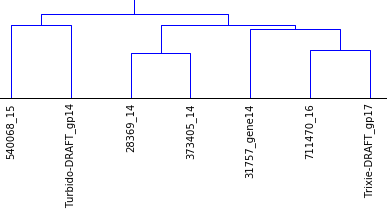
\includegraphics[scale=0.7]{img/tree_fig_4}
		\caption{Tree sub-selection}
	\end{center}
\end{figure}

The figure 5.1 is a selection from figure 3.20. It will be interesting to extend the function in figure 4.1 to select those sub-parts. Wether listing all the sub-parts, wether by selecting a part from a specific gene.

\addtocounter{chapter}{1}
\addcontentsline{toc}{chapter}{\protect\numberline{\thechapter}List of figures}
\listoffigures

\addtocounter{chapter}{1}
\addcontentsline{toc}{chapter}{\protect\numberline{\thechapter}References}
\bibliographystyle{plain} % Le style est mis entre accolades.
\bibliography{bibli} % mon fichier de base de données s'appelle bibli.bib


\chapter{Annexes}
\begin{enumerate}
	\item \textbf{phages\_list\_1.txt}
	\item \textbf{phamerator.sh}
	\item \textbf{respham2799hoststrain.pdf}
	\item \textbf{SEA.sql}
	\item \textbf{show\_phamily.ipynb.pdf}
	\item \textbf{GeneBank\_Fetch.ipynb.pdf}
\end{enumerate}


\end{document}



